%\title{Project Report}
%
%%% Preamble
\documentclass[paper=a4, fontsize=11pt]{scrartcl}
\usepackage[T1]{fontenc}
\usepackage{fourier}

\usepackage[english]{babel}															% English language/hyphenation
\usepackage[protrusion=true,expansion=true]{microtype}
\usepackage{amsmath,amsfonts,amsthm} % Math packages
\usepackage[pdftex]{graphicx}
\usepackage{url}
\usepackage{listings}
\usepackage[final]{pdfpages}
\usepackage[section]{placeins}

%%% Custom sectioning
\usepackage{sectsty}
\allsectionsfont{\centering \normalfont\scshape}


%%% Custom headers/footers (fancyhdr package)
\usepackage{fancyhdr}
\pagestyle{fancyplain}
\fancyhead{}											% No page header
\fancyfoot[L]{}											% Empty
\fancyfoot[C]{}											% Empty
\fancyfoot[R]{\thepage}									% Pagenumbering
\renewcommand{\headrulewidth}{0pt}			% Remove header underlines
\renewcommand{\footrulewidth}{0pt}				% Remove footer underlines
\setlength{\headheight}{13.6pt}


%%% Equation and float numbering
\numberwithin{equation}{section}		% Equationnumbering: section.eq#
\numberwithin{figure}{section}			% Figurenumbering: section.fig#
\numberwithin{table}{section}				% Tablenumbering: section.tab#


%%% Maketitle metadata
\newcommand{\horrule}[1]{\rule{\linewidth}{#1}} 	% Horizontal rule

\title{
		%\vspace{-1in}
		\usefont{OT1}{bch}{b}{n}
		\normalfont \normalsize \textsc{University of Michigan} \\ [25pt]
		\horrule{0.5pt} \\[0.4cm]
		\huge AERO 584, Homework  7 \\
		\horrule{2pt} \\[0.5cm]
}
\author{
		\normalfont 								\normalsize
         Huckleberry Febbo\\[-3pt]		\normalsize
        \today
}
\date{}

%%%%%%%%%%%%%%%%%%%%%%%%%%%%%%%%%%%%%%%%%%%%%%%%%%%%%%%%%%%%%%%%%%%%%
%%%%%%%%%%%%%%%%%%%%%%%%%%%%%%%%PACKAGES%%%%%%%%%%%%%%%%%%%%%%%%%%%%%%%%

% *** MATH ***
\usepackage{amsmath}
\usepackage{cases}
\usepackage{mathrsfs}
\usepackage{amssymb}
\DeclareMathAlphabet\mathbfcal{OMS}{cmsy}{b}{n}


% *** GRAPHICS ***
\usepackage[]{graphicx}
\usepackage{epstopdf}
\usepackage{svg}
\setsvg{inkscape=inkscape -z -D,svgpath=figs/}

\usepackage{lineno,hyperref}
\modulolinenumbers[5]


\bibliographystyle{elsarticle-num}
%%%%%%%%%%%%%%%%%%%%%%%

\begin{document}
\maketitle
\section*{Problem 5.1}

Following the derivation for Pursuit Guidance from page 121-123 in the book Eqn. (5.19) can be extended to higher order derivatives as follows. First for this scheme, we first set $\theta = \beta$, next the established pattern for finite derivatives is studied:\\
For k = 1:\\
$$\gamma \leq 2=\frac{1+1}{1}$$
For k = 2:\\
$$\gamma \leq \frac{3}{2}=\frac{2+1}{2}$$

Thus, for any k:\\
$$\gamma \leq \frac{k+1}{k}$$

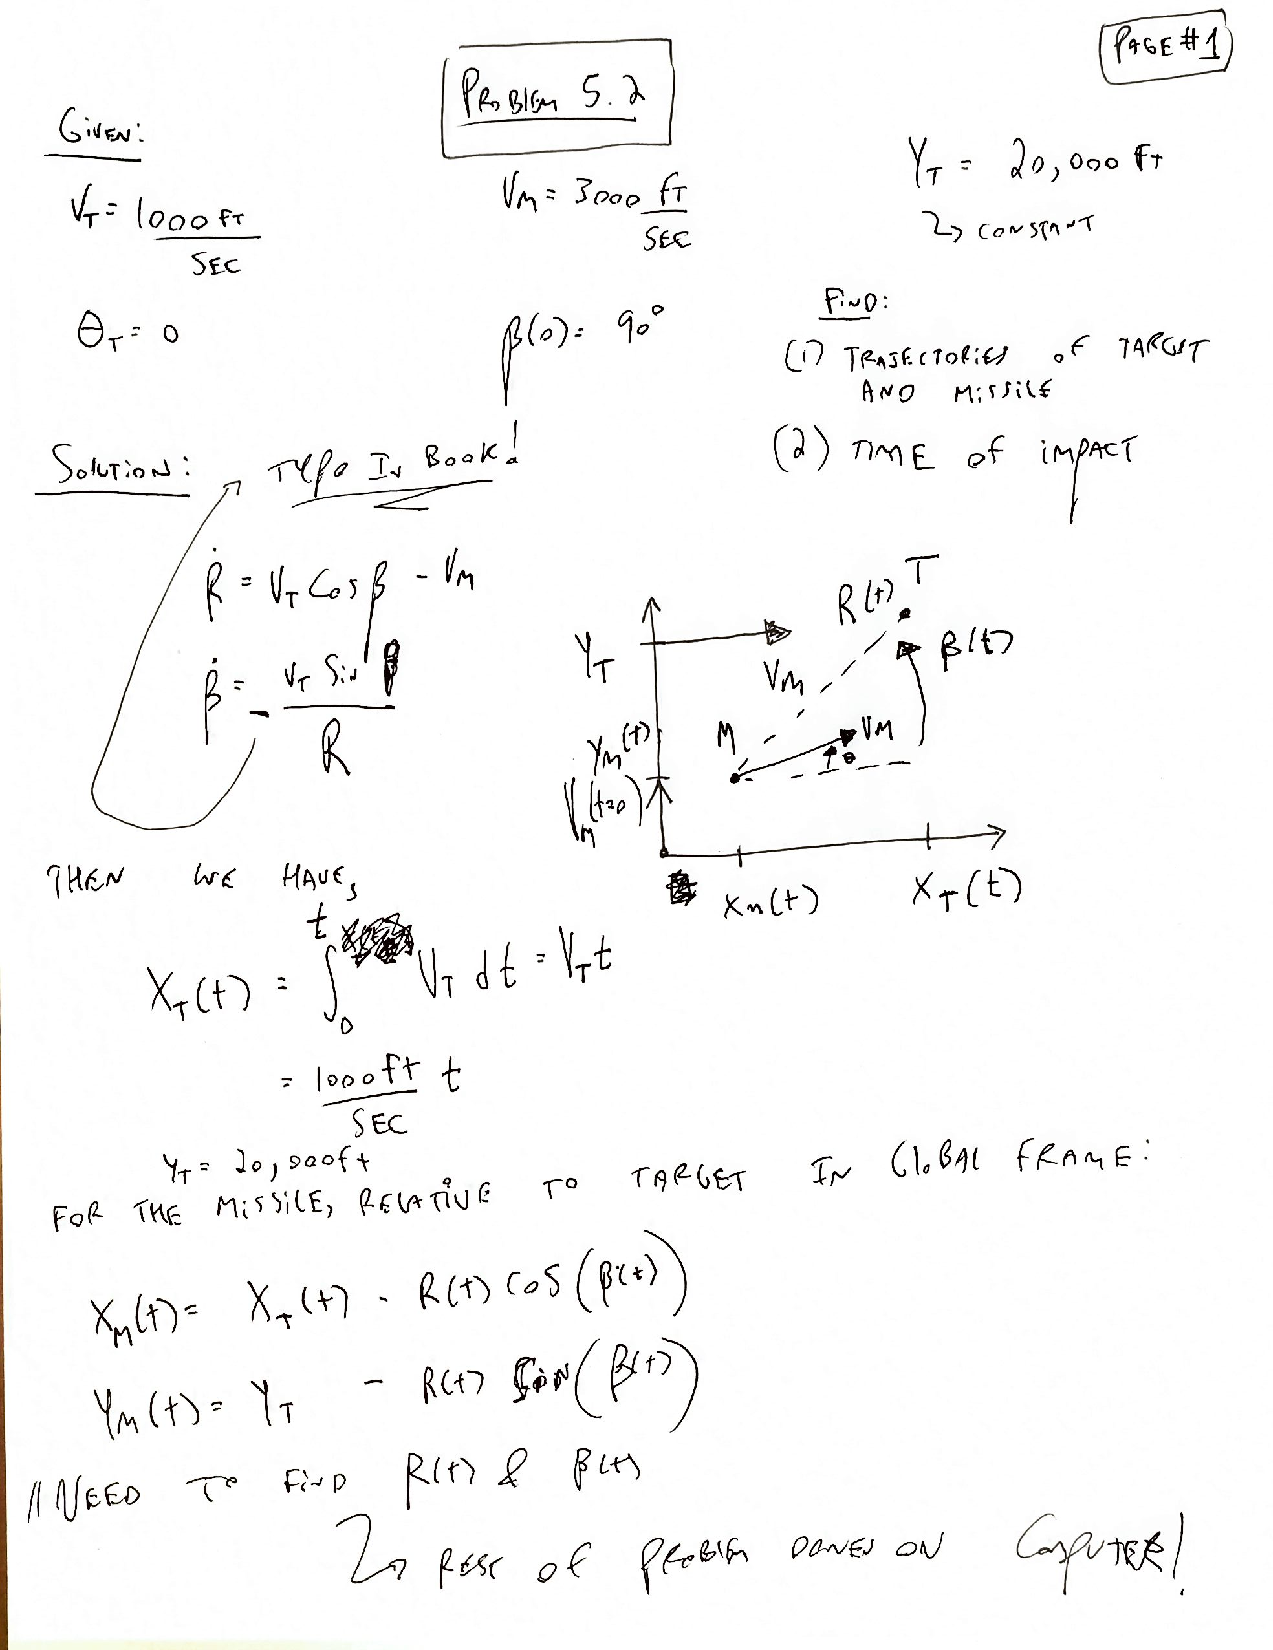
\includepdf[pages=-]{a.pdf}


\begin{figure}[!htb]
	\centering
    \includesvg[width=0.9\textwidth]{p2}
	\caption{ \label{fig:f1}}
\end{figure}

\section*{Problem 5.3}
%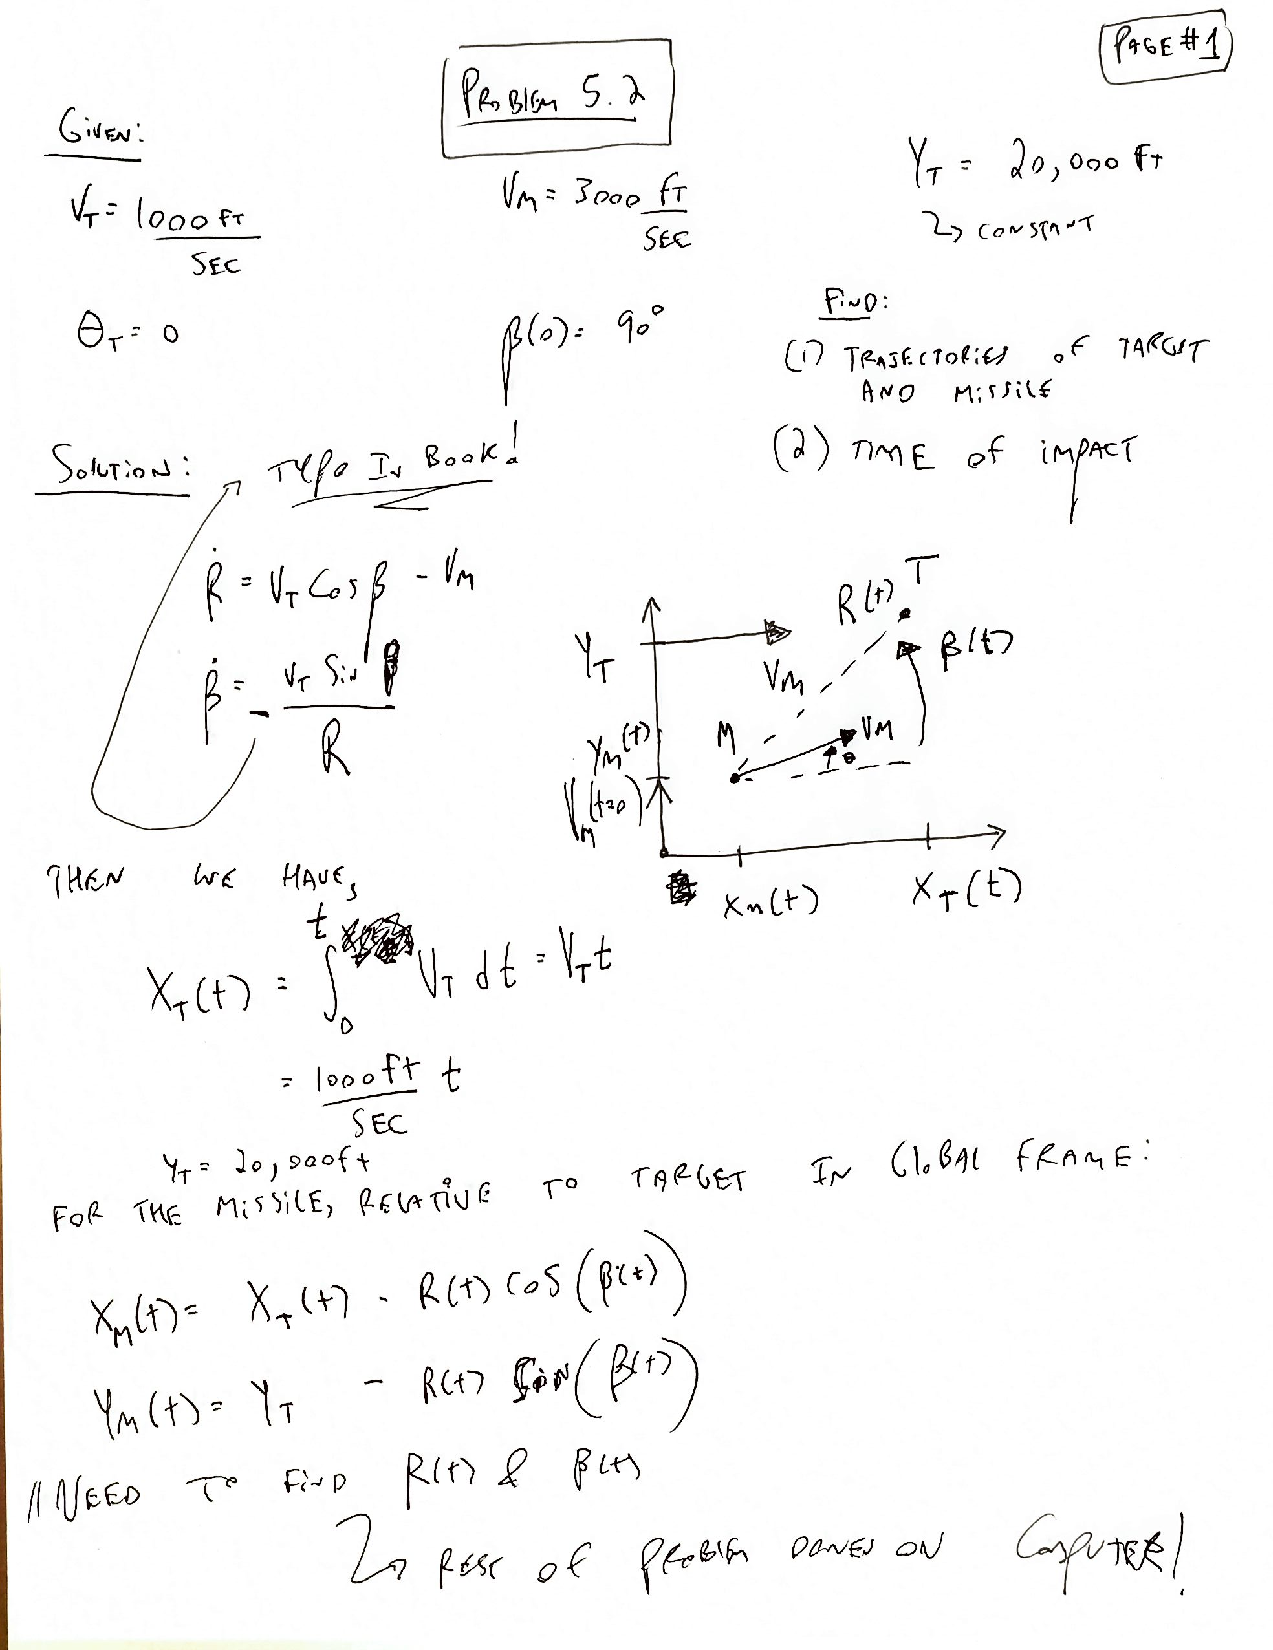
\includepdf[pages=-]{a.pdf}

NOTE:  $\theta = \beta$ for pursuit guidance \\

As seen in Fig. \ref{fig:f3} the trajectory is rate limited where it stops, which is at $t=6.79$. If integration where to continue it would go behind the target and miss it. But, it cannot continue because the differential equations become unstable as $t \rightarrow t_f$ because $\dot{\beta} \rightarrow \infty$ as can be seen in Fig. \ref{fig:f3b}. Which is is approximately\footnote{ approximately because the differential equation given for $\ddot{\beta}$ is only good for $\beta << 1$ which is not the case} the time where we will go to our acceleration limit. 

\begin{figure}[!htb]
	\centering
    \includesvg[width=0.9\textwidth]{p3}
	\caption{ \label{fig:f3}}
\end{figure}

\begin{figure}[!htb]
	\centering
    \includesvg[width=0.9\textwidth]{p3b}
	\caption{ \label{fig:f3b}}
\end{figure}

To find the miss distance, a new set of differential equations where solved (see code) where a state was added $\ddot{\beta}$ which was set to $40\times32.2$ \footnote{the maximum turning acceleration} and then $\dot{\beta}$ was set to itself (now that it has been included as a state). Then integration was picked up where Fig. \ref{fig:f3} left off.   These trajectory results are shown in Fig. \ref{fig:f3c} where the missile missed the target given rate limit shown in Fig. \ref{fig:f3e}. The miss distance is calculated as the minimum of R, because that is the closest that the missile got to the target, the result is shown in Fig. \ref{fig:f3d} 
\begin{figure}[!htb]
	\centering
    \includesvg[width=0.9\textwidth]{p3c}
	\caption{ \label{fig:f3c}}
\end{figure}

\begin{figure}[!htb]
	\centering
    \includesvg[width=0.9\textwidth]{p3d}
	\caption{ \label{fig:f3d}}
\end{figure}

\begin{figure}[!htb]
	\centering
    \includesvg[width=0.9\textwidth]{p3e}
	\caption{ Missile hits acceleration limit at about 2 seconds. This does not match what was predicted in Fig. \ref{fig:f3b}, but different integration schemes where used. In this investigation a simple one was used, see code\label{fig:f3e}}
\end{figure}

\section*{Problem 5.4}
%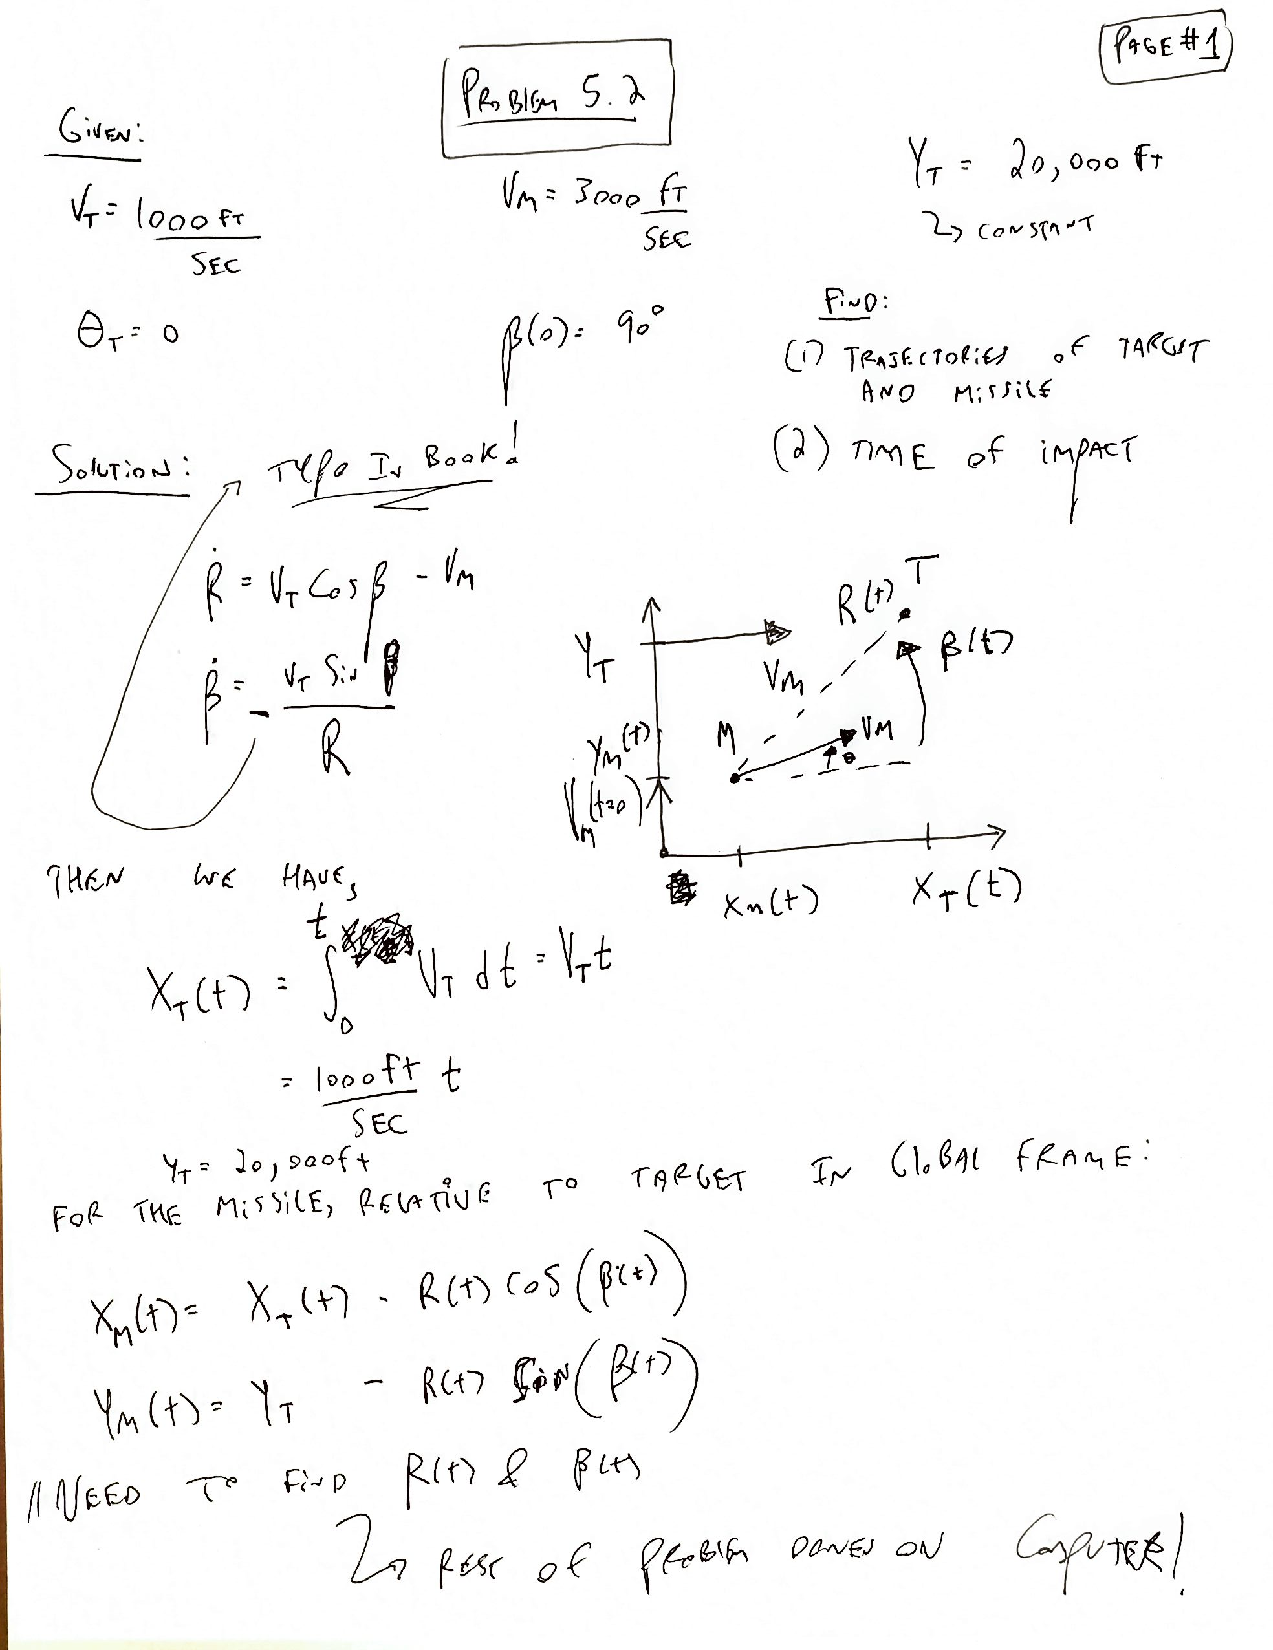
\includepdf[pages=-]{a.pdf}
For fixed lead guidance we have
$$\frac{V_m}{sin(\beta_0-\theta_m)}=\frac{V_t}{sin(\beta_0-\theta_t)}$$

where $\beta_0=\frac{\pi}{2}$, $V_m=1000 \frac{ft}{s}$, $V_t=1000 \frac{ft}{s}$, and $R(0)=2000ft$ \\

For the missile to collide, it needs to be headed with the angle, $$ \theta_m = acos(\frac{1}{3}) = 1.23 rad$$ The time to impact is shown in Fig. \ref{fig:f4} as $tf =7.08 s$
\begin{figure}[!htb]
	\centering
    \includesvg[width=0.9\textwidth]{p4}
	\caption{ \label{fig:f4}}
\end{figure}

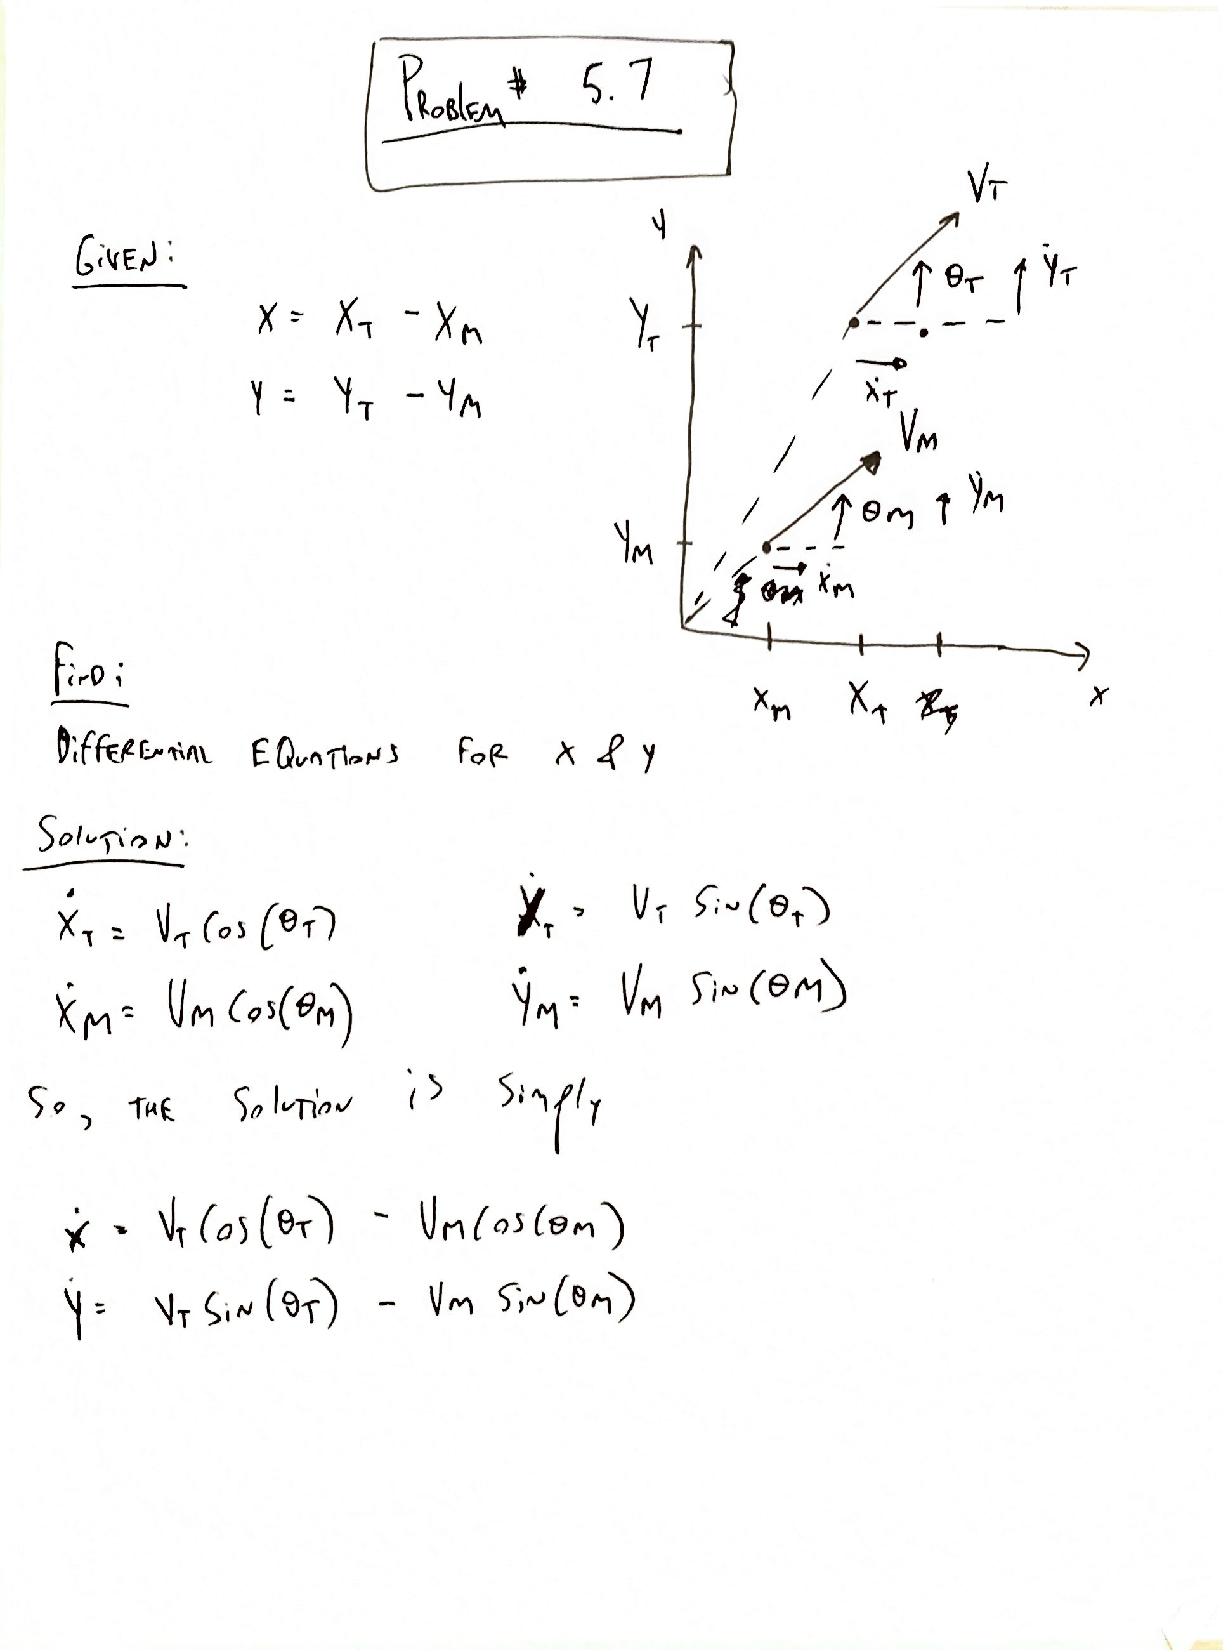
\includepdf[pages=-]{b.pdf}
\section*{code for 5.2 and 5.3}
\begin{lstlisting}
using Plots
pgfplots()
using LaTeXStrings
PGFPlots.pushPGFPlotsPreamble("\\usepackage{amssymb}")
using OrdinaryDiffEq
using DiffEqBase
#using ParameterizedFunctions
using DiffEqCallbacks

TT = linspace(0,10,1000)
const Vt = 1000;
const Vm = 3000;

# differential equations
f = (t,x,dx) -> begin

     # diff eqs.
     dx[1] = Vt*cos(x[2])-Vm;      # 1. R
     dx[2] = -Vt*sin(x[2])/x[1];   # 2. B
end

x0 = [20000;pi/2]
tspan = (TT[1],TT[end])
prob = ODEProblem(f,x0,tspan)
sol = DiffEqBase.solve(prob,Tsit5())

# extract results
x1 = [sol(t)[1] for t in TT]
x2 = [sol(t)[2] for t in TT]

Xm = zeros(length(TT),1); Ym = zeros(length(TT),1);
Xt = zeros(length(TT),1); Yt = 20000*ones(length(TT),1);
tf=0;num=0;
for i in 1:length(TT)
     Xt[i] = Vt*TT[i]
     Xm[i] = Xt[i] - x1[i]*cos(x2[i])
     Ym[i] = 20000 - x1[i]*sin(x2[i])
     if Ym[i] > 20000
          tf = TT[i]
          num = i
          break
     end
end

# misc variables
l1 = (4,:red,:solid)
l2 = (3,:green,:solid)
l3 = (2,:black,:dot)

s1 = string("missle, with impact time = ",round(tf,2))
s2 = "target"

# position
p1 = plot(Xm[1:num],Ym[1:num],line=l1,label=s1)
plot!(Xt[1:num],Yt[1:num],line=l2,label=s2)
yaxis!("y (m)")
xaxis!("x (m)")
savefig(string("figs/p2",".",:svg));

# prob 5.3, amy_max = 40*32.2
# since theta = beta for pursuit guidance
c = 670
c2 = c-1
c3=1000
const g = Vm/Vt
const tf_g = TT[c]
const b0 = pi/2
const TM = 40*32.2
# differential equations
f = (t,x,dx) -> begin

     # diff eqs.
     dx[1] = Vt*cos(x[2])-Vm;      # 1. R
     dx[2] = -Vt*sin(x[2])/x[1];   # 2. B - > dx[3] does not work here because B is not << 1
     dx[3] = b0*(2-g)/((g-1)^2*(tf_g)^2)*((tf_g-t)/(tf_g))^((3-2*g)/(g-1))  # unstable because Bdot goes to infinity as t goes to tf
end

x0 = [20000;pi/2;0]
tspan = (TT[1],TT[c2])
prob = ODEProblem(f,x0,tspan)
sol = DiffEqBase.solve(prob,Tsit5())

# extract results
ff=indmin(abs.(sol.t[end] - TT))-1

x1 = [sol(t)[1] for t in TT[1:ff]]
x2 = [sol(t)[2] for t in TT[1:ff]]
x3 = [sol(t)[3] for t in TT[1:ff]]

Xml = zeros(length(TT),1); Yml = zeros(length(TT),1);
Xt = zeros(length(TT),1);
tf2 = 0;num2=0;
for i in 1:ff
     Xt[i] = Vt*TT[i]
     Xml[i] = Xt[i] - x1[i]*cos(x2[i])
     Yml[i] = 20000 - x1[i]*sin(x2[i])
     tf2 = TT[i]
     num2 = i
     if Yml[i] > 20000
          break
     end
end

s1 = string("missle, with impact time = ",round(tf,2))
s2 = "target"
s3 = string("missle, with miss")

# position
p1 = plot(Xm[1:num],Ym[1:num],line=l1,label=s1)
plot!(Xt[1:num],Yt[1:num],line=l2,label=s2)
plot!(Xml[1:num2],Yml[1:num2],line=l3,label=s3,legend=:bottomright)
yaxis!("y (m)")
xaxis!("x (m)")
savefig(string("figs/p3",".",:svg));

# turning rate
p1 = plot(TT[1:ff],x3[1:ff],line=l1)
yaxis!("Beta Dot")
xaxis!("t (s)")
savefig(string("figs/p3b",".",:svg));


#####################
## finding Ym
Xml = zeros(length(TT),1); Yml = zeros(length(TT),1);
Xt = zeros(length(TT),1);
x1 = zeros(length(TT),1);
x2 = zeros(length(TT),1);
x3 = zeros(length(TT),1);
x4 = zeros(length(TT),1);

# inital conditions
Yt[1] = 20000
x1[1] = 20000
x2[1] = pi/2
for i in 1:length(TT)-1
     dt = TT[i+1]-TT[i]
     Xt[i+1] = Xt[i] + Vt*TT[i]*dt
     Xml[i+1] = Xml[i] + Vm*cos(x2[i])*dt
     Yml[i+1] = Yml[i] + Vm*sin(x2[i])*dt
     x1[i+1] = sqrt((Yt[i]-Yml[i])^2 + (Xt[i]-Xml[i])^2)
     x2[i+1] = atan2(Yt[i]-Yml[i],Xt[i]-Xml[i]) # beta
     x3[i+1] = x3[i] + (x2[i+1] - x2[i])/dt # beta dot
     x4[i+1] = x4[i] + (x3[i+1] - x3[i])/dt # beta double dot
     if x4[i+1] > TM
          x4[i+1] = TM
     elseif x4[i+1] < -TM
          x4[i+1] = -TM
     end
end

s1 = string("missle, with impact time = ",round(tf,2))
s2 = "target"
s3 = string("missle, with miss")

# position
num2 = 1000
p1 = plot(Xm[1:num],Ym[1:num],line=l1,label=s1)
plot!(Xt[1:num],Yt[1:num],line=l2,label=s2)
plot!(Xml[1:num2],Yml[1:num2],line=l3,label=s3,legend=:bottomright)
yaxis!("y (m)")
xaxis!("x (m)")
savefig(string("figs/p3c",".",:svg));

# miss distance
Ym=x1[indmin(abs.(x1))]
tm=TT[indmin(abs.(x1))]
p1 = plot(TT,x1,line=l1,label=string("Ymiss = ",round(Ym,2)," (m); at t = ",round(tm,2), " (s)" ))
yaxis!("Ym (m)")
xaxis!("t (s)")
savefig(string("figs/p3d",".",:svg));

# miss distance
p1 = plot(TT,x4,line=l1)
yaxis!("Turning Acceleration")
xaxis!("t (s)")
savefig(string("figs/p3e",".",:svg));

\end{lstlisting}



\section*{code}
\begin{lstlisting}


\end{lstlisting}




\section*{code}
\begin{lstlisting}


\end{lstlisting}

\end{document}
